\twocolumn
\begin{figure}[h]
    \centering
    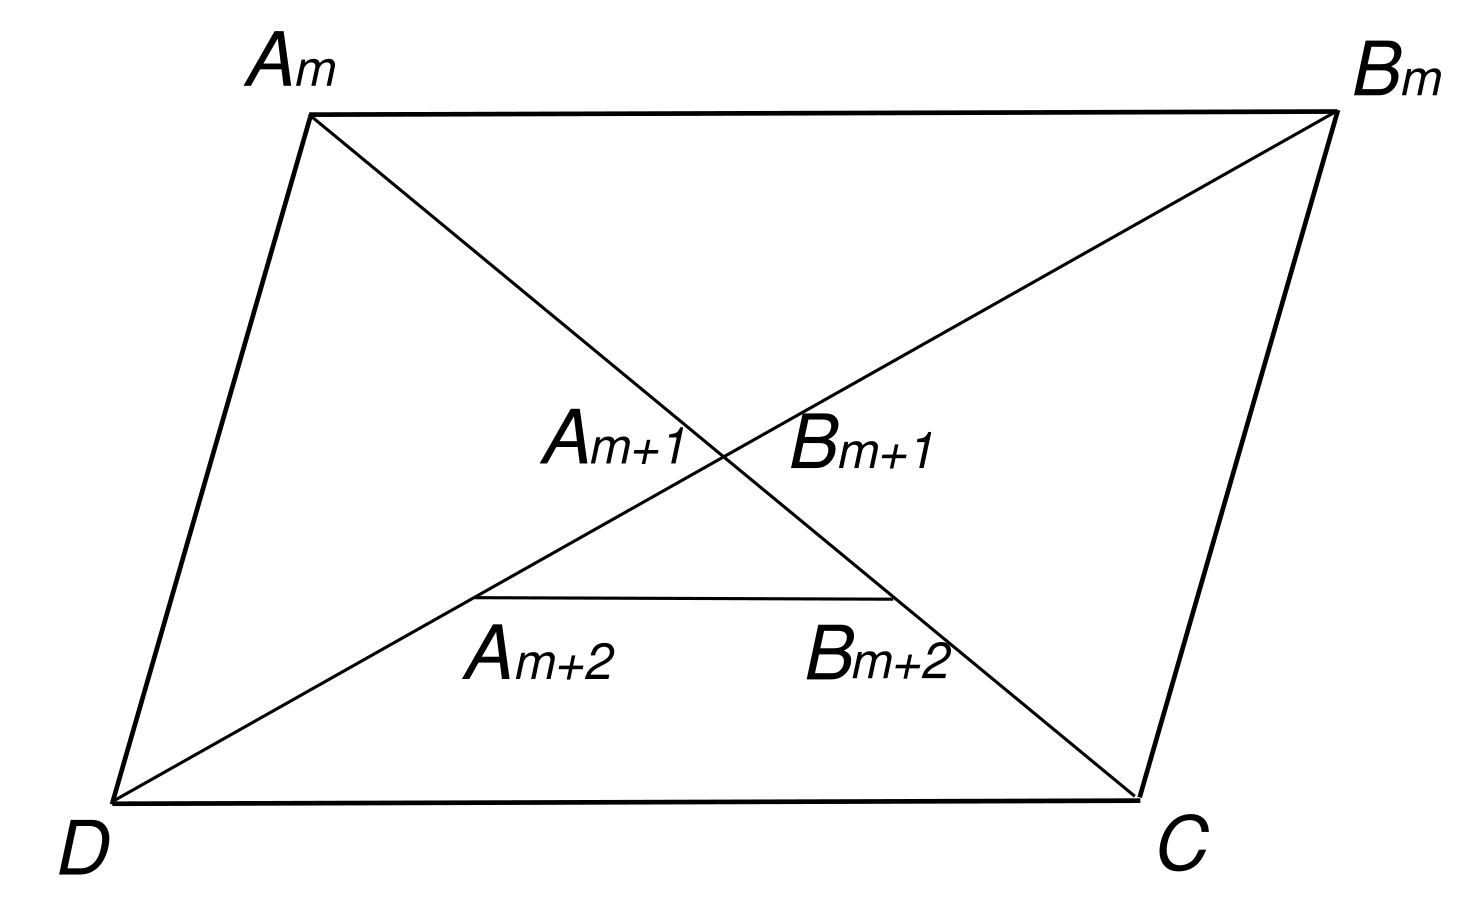
\includegraphics[width=\linewidth]{piped.png}
    \begin{flushleft}
    \textbf{Рисунок 5.}
    \end{flushleft}
\end{figure}
К сожалению, некоторые читатели пишут: <<Поскольку последовательность не монотонная, она не стремится к пределу>>. Это рассуждение, конечно, неверно. Докажем строго, пользуясь определением предела, что \[\lim_{n\to\infty} a_n = \frac{b}{3}. \tag{4} \label{first}\] \par Пусть задано $\varepsilon>0$. Тогда если $n>N$, где $N = N_{(\varepsilon)}$ -- наименьшее целое число, для которого $2^N\varepsilon> 2^m|\delta_m|$, то $|a_n -\frac{b}{3}| = |\delta_n| =  \frac{|\delta|}{2^{n-m}} < \frac{|\delta_m|}{2^{N-m}} < \varepsilon$.\\ Тем самым \eqref{first} доказано. \par
Разумеется, предел равен $\frac{b}{3}$ и в том случае, когда $a_m = \frac{b}{3}$ -- в этом случае все последующие члены тоже равны $\frac{b}{3}$. Выясним, при каких значениях $a$ возникает этот случай. Если $m=0$, то $a=\frac{b}{3}$. Если $m=1$ и $a_1 = \frac{a-b}{2} = \frac{b}{3}$, то $a=\frac{5b}{3}$.\\
\begin{figure}[h]
    \centering
    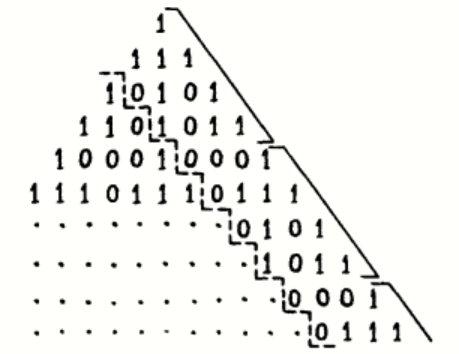
\includegraphics[width=\linewidth]{ktexu.png}
    \begin{flushleft}
    \textbf{Рисунок 6.}
    \end{flushleft}
\end{figure}\\
Вообще, если $a_m = \frac{b}{3}$, то $a=a_0$ получается из $a_m=\frac{b}{3}$ после $m$-кратного применения формулы $a_{n-1} = 2a_n+b$. Таким образом, как нетрудно проверить, значения $a$, при которых $a_m = \frac{b}{3}$, составляют последовательность $\frac{b}{3}$, $\frac{5b}{3}$, $\frac{13b}{3}$, . . . , $\frac{(2^k-3)b}{3}$, . . . При всех (и только этих) значениях $a$ последовательность получается монотонной (и с некоторого места -- постоянной). \par Мы не выделили случай, когда $a_m = b$ (при этом $a_{m+1} = 0$, $a_{m+2}=\frac{b}{2}$, . . .), -- с алгебраической точки зрения он ничем не примечателен, но соответствующие $n=m$ и $n=m+1$ трапеции вырождаются в параллелограмм и в треугольник (точки $B_{m+1}$ и $C_{m+1}$ совпадают); начиная с $n=m+2$, получаются настоящие трапеции, и, как всегда, $a_n$ стремится к пределу $\frac{b}{3}$.
\begin{center}
    \large \textbf{M98}
\end{center}
\par Докажите, что в таблице\\
\begin{center}
\begin{tabularx}{0.6\linewidth}{
>{\centering\arraybackslash}X
>{\centering\arraybackslash}X
>{\centering\arraybackslash}X
>{\centering\arraybackslash}X
>{\centering\arraybackslash}X
>{\centering\arraybackslash}X
>{\centering\arraybackslash}X
>{\centering\arraybackslash}X
>{\centering\arraybackslash}X
}
    &&&&1&&&&&
    &&&1&1&1&&&&
    &&1&2&3&2&1&&&
    &1&3&5&7&6&3&1&&
    .&.&.&.&.&.&.&.&.&
\end{tabularx}
\end{center}
где каждое число равно сумме трёх, стоящих над ним, в каждой строке (начиная с третьей) есть чётное число. В каждой ли строке (кроме первых двух) встречается число, делящееся на три?\par Исследуем сначала вопрос о делимости на два. Будем в нашей таблице вместо чётных чисел писать 0, а вместо нечётных -- 1. Тогда таблицу 0 и 1 нужно будет составлять по тому же правилу (каждое число получается как сумма трёх, стоящих над ним в предыдущей строке), только сложение нужно выполнять <<по модулю два>> -- по правилам $0+0=0$, $0+1 = 1+0 =1$, $1+1 = 0$. \par Первое решение основано на таком соображении: последние четыре числа в каждой строке зависят только от того, каковы последние четыре числа в предыдущей строке, и поэтому нет ничего удивительного в том, что эта четвёрка переодически повторяется (с периодом 4, см. рисунок 6) *)
\par Другое решение, предложенное рядом читателей -- доказательство от противного. Предположим, что какая-то строка целиком состоит из единиц: $$111{\,....\,....\,}111$$
Тогда предыдущая строка, как легко убедиться, может быть только такой:
$$100100{...\,...}001001{,}$$
а идущая перед ней -- только такой:
$$110000110000{\,...\,...\,}000011000011{.}$$
\\
------------
\par )* Аналогичное решение приводится в книге Дs. О. Ш~к~л~я~р~с~к~о~г~о, Н. Н. Ч~е~ч~е~н~ц~о~в~а и И. М. Я~г~л~о~м~а <<Избранные задчачи и теоремы элементарной математики>>, изд. 4-е, <<Наука>>, 1965, задача 10.